\documentclass[../main.tex]{subfiles}

% Importing images from another path
\graphicspath{{\subfix{../images/}}}

\begin{document}

In order to better understant the models presented in this report, it's first necessary to briefly explain how the studied algorithms for the modelled collective operations work.\\
The two collective operations studied in this work are the \textbf{broadcast} operation, where a single process (the root) sends the same message to all processes, and the \textbf{reduce} operation, where all processes send their data to a single process (the root) that aggregates them.\\
\textit{OpenMPI} architecture is based on a modular approach where different software components, plugged in the library kernel, provide specific implementation features. The \cc{tuned} component, in particular, is responsible for the selection of different algorthms for a particular collective operation. Since an MPI collective operation can be seen as a set of point-to-point tranmission between processes, the algorithms differ one from the other in the way they manage these point-to-point communications. In the case of this study, a total of $4$ different algorithms have been considered for both operations.\\
First of all, the \textbf{default} algorithm has been used for both operation as a baseline. In MPI, the default algorithm has no precise implementation since the library itself decides at runtime one of the many possible algorithms available for the specific collective operation requested, based on a decision routine.\\
The \textbf{linear} algorithm, also known as \textbf{flat tree} algorithm, has then been taken into account for this study. As depicted in figure~\ref{fig:algorithms}a, this algorithm translates into a single level tree topology where the root has $P-1$ children and the message is sent (received)\footnote{This refers to the broadcast case, between brackets the analogous for the reduce one.} to (from) children processes without segmentation.
Since \textit{OpenMPI} implements this algorithm using non-blocking send and blocking receive point-to-point communications, the tree topology of this algorithm is known in literature as a \textit{Non-Blocking Fat Tree (NBFT)}~\cite{Nuriyev2022}. The execution time $T^{c}_{NBFT}(P,m)$ of such algorithm, while transmitting a message of size $m$ to $P-1$ processes throught a channel of communication $c$, can be upper bounded by the execution time $T^{c}_{BFT}(P,m)$ of its \textit{Blocking Fat Tree (BFT)} counterpart, which only uses blocking send-receive communications. At the same time, $T^{c}_{NBFT}(P,m)$ must logically be greater or equal to the time of a single point-to-point communication, hence the following inequality holds:
\begin{equation}\label{eq:nbft-inequality}
    T^{c}_{p2p}(m) \leq T^{c}_{NBFT}(P,m) \leq T^{c}_{BFT}(P,m) = (P-1) \cdot T^{c}_{p2p}(m)
\end{equation}
where $T^{c}_{p2p}(m)$ is the time of a single point-to-point communication transmitting a message of size $m$ through channel $c$.\\
The third algorithm considered has been the \textbf{chain} algorithm. In this case, each node of the topology has one child, therefore the message is split in $n_s$ segments of size $m_s$ and transmission of segments continues in a pipeline where process $i$ sends (receives) segments to (from) process $i+1$. Therefore, this algorithm describes a chain tree of height $P-1$, that can be completed in $P+n_s-2$ sequential stages. Since each stage consists of multiple concurrent NBFTs of $P=2$ nodes, as shown in figure~\ref{fig:algorithms}b, the overall execution time of the algorithm will be equal to the sum of the maximum times $T^{c_i}_{NBFT}(2,m_s)$ of each $i^{th}$ stage.
\begin{equation}\label{eq:chain-time}
    T_{chain}(P,m,n_s) = \sum_{i=1}^{P+n_s-2} \underset{j_i}{\max}\; T^{c_{j_i}}_{NBFT}(2,m_s)
\end{equation}
Where $c_{j_i}$ is the communication channel of the $j^{th}$ NBFT running at the $i^{th}$ stage.\\
The last algorithm studied is the \textbf{binary tree} algorithm (figure~\ref{algorithms}c). As the name suggests, this algorithm is represented by a binary tree where each node $i$ exchanges segmented messages with two children $2i$ and $2i+1$. Assuming for simplicity that the tree is complete, then its height will be $\lfloor\log_2(P)\rfloor$ and the algorithm will be completed in $\lfloor\log_2(P)\rfloor+n_s-1$ stages, each cosisting of multiple NBFT of either $2$ or $3$ nodes. Therefore, in this case:
\begin{equation}\label{eq:binary-time}
    T_{binary}(P,m,n_s) = \sum_{i=1}^{\lfloor\log_2(P)\rfloor+n_s-1} \underset{j_i}{\max}\; T^{c_{j_i}}_{NBFT}(P_i,m_s)
\end{equation}
Where the number of NBFTs changes at each stage, starting from $1$ from stage $1$ and reaching a maximum of $2^{\lfloor\log_2(P)\rfloor}$ in the middle stages.\\

% \begin{figure}[h]
%     \centering
%     \subfloat[Linear algorithm]{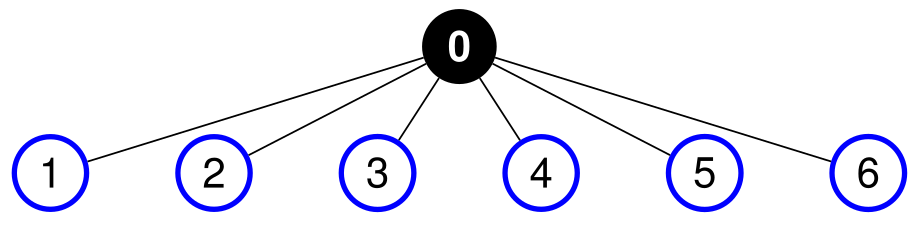
\includegraphics[width=0.3\textwidth]{linear-fat-tree.png}}
%     \subfloat[Chain algorithm]{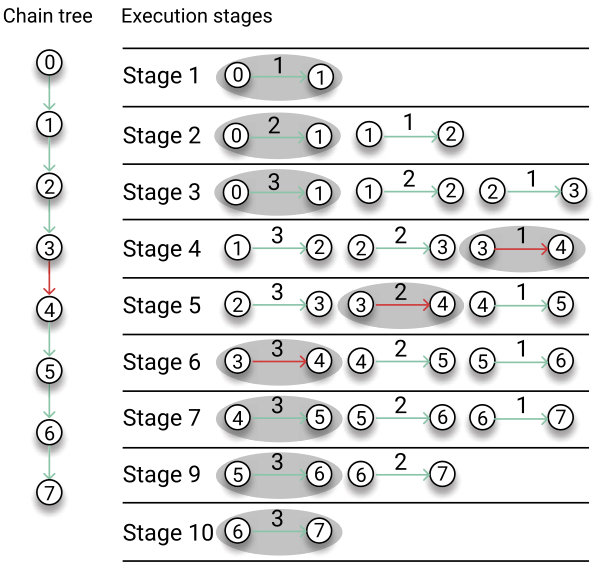
\includegraphics[width=0.3\textwidth]{chain-fat-tree.png}}
%     \subfloat[Binary tree algorithm]{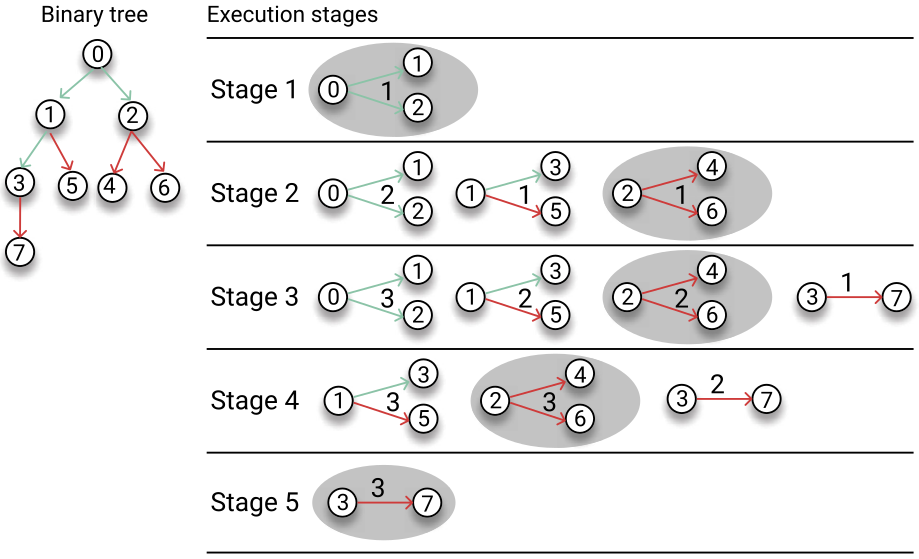
\includegraphics[width=0.3\textwidth]{binary-fat-tree.png}}
%     \caption{Schematic representation of the studied algorithms}
%     \label{fig:algorithms}
% \end{figure}

\begin{figure}[h]
    \centering
    \begin{minipage}{\textwidth}
        \centering
        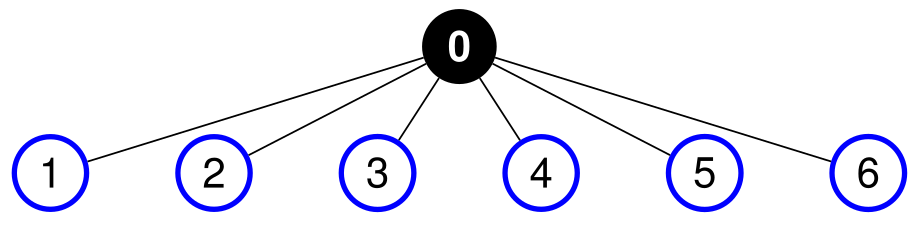
\includegraphics[width=0.6\textwidth]{linear-fat-tree.png}
        \subcaption{Linear algorithm}
    \end{minipage}
    
    \begin{minipage}{0.4\textwidth}
        \centering
        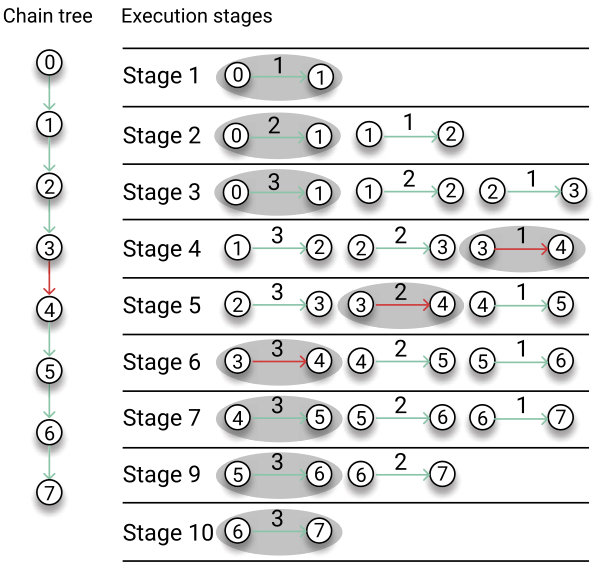
\includegraphics[width=0.9\textwidth]{chain-fat-tree.png}
        \subcaption{Chain algorithm}
    \end{minipage}\hfill
    \begin{minipage}{0.6\textwidth}
        \centering
        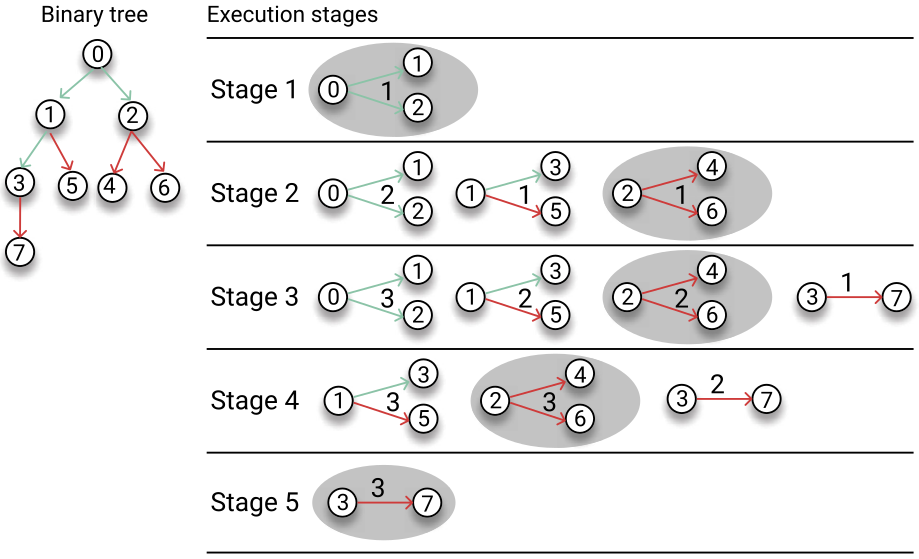
\includegraphics[width=0.9\textwidth]{binary-fat-tree.png}
        \subcaption{Binary tree algorithm}
    \end{minipage}
    \caption{Schematic representation of (a) linear, (b) chain and (c) binary tree algorithms.}
    \label{fig:algorithms}
\end{figure}

Equation~\ref{eq:nbft-inequality} allows to approximate the execution time of a NBFT as follows:
\begin{equation}\label{eq:nbft-approx}
    T^{c}_{NBFT}(P,m) \approx \gamma^{c}(P,m) \cdot T^{c}_{p2p}(m)
\end{equation}
where $\gamma^{c}(P,m)$ is a \textit{parallelization factor}, representing the increase in latency of $P-1$ concurrent point-to-point communications in channel $c$, originating from the same root and transmitting a message of size $m$, with respect to a single point-to-point communication. Starting from this approximation, is therefore possible to build a model for the prediction of collective operations latencies based on single point-to-point communications latencies as it'll be explained in the next sections. In fact, the ability of predicting the latency of an arbitrairly large NBFT makes also possible to extend the model for predicting latencies of the previously introduced algorithms thanks to equations~\ref{eq:chain-time} and~\ref{eq:binary-time}.\\

\end{document}